\section{Introduction}

The optimization of quantum circuit has various meaning by the contenxt. 
In this section, the term \textit{optimization} is used as indicating two concept.
First is error reducing technique of circuit representation of time-evolution dynamics, 
and Second is a direct circuit depth reduction techniques.

\section{Mutally commuting groups}

In the Product formula, Eq(\ref{eq:product_formula}), 
the total time evolution operator is approximated with product of several local Hamiltonian operators.
It is just an approximation but actively adopted in many references and methods. % Trotter formula reference 와 QAOA 방법론 언급
The reason is that we don't know proper method to find exact evolution operator corresponding to the total Hamiltonian.
Moreover, the method represents the locality of the given system well. % cite trotter error paper.
In such representation, the product order of local operators does not affect the \textit{physical} system or 
ther is no dependence on the system.
It is purely error reduction technique of the implementation.

Start from the 3 terms, $A, B, C$ hermite operators, 
the given Hamiltonian is $H = A +  B +  C$.
By the BCH formula, the product of $\exp(A) \exp(B) \exp(C)$ has next error terms.

\begin{eqnarray}
    \exp(A)\exp(B) &=& \exp(A+B) \exp(\Theta(A, B))\\
    \exp(A + B)\exp(C) &=& \exp(A + B + C) \exp(\Theta((A+ B), C))\\
    \exp(A)\exp(B)\exp(C) &=& \exp(A+B+C) \exp(\Theta((A+B), C) - \Theta(A, B)) 
\end{eqnarray}

However, the error term $\Theta(A, B) = \Theta([A, B])$ and $\Theta(0) = 0$,
it means that in the case of commuting operators $[A, B] = [B, C] = [A, C] = 0$, 
the product formula is exactly same the proper time evolution operator,

\begin{equation}
    \exp(A)\exp(B)\exp(C) = \exp(A + B + C)
\end{equation}

It is not a general case of the simulation, however, there are mutually commuting subsets exists generally.
The situation of every local Hamitlonians are anti-commuting each other is also a rare case as much as the all commuting case.

Childs et al derived product formula error with commutator scaling\cite{PhysRevX.11.011020}.

\begin{theorem}\textbf{Product error with commutator scaling}
    
    Let, $\mathcal{L}_p(H, t)$ be a $p$-th order product formula of the given Hamiltonian, $H = \sum_i H_i$.
    Then, the error of the $p$-th order approximation is 

    \begin{equation}
        \| \mathcal{L}_p(H ,t) - \exp(-i t H) \| = \mathcal{O}(\tilde{\alpha}_{com} t^{p+1}),
    \end{equation}
    where, $\tilde{\alpha}_{com} := \sum_{\lambda_1, \lambda_2, \dots , \lambda_{p+1}} \Vert[H_{\lambda_{p+1}}, \dots [H_{\lambda_2}, H_{\lambda_1}]] \Vert$
    
\end{theorem}

The reduction of big-O error does not significantly large, however, mutually commuting group allow us some freedom to manipulate additional optimization about the circuit gates.

\section{Hamiltonian grouping problem}

We can construct a graph of which edges are indicating commuting, anti-commuting relathion of Pauli nodes.
Such graph is called \textit{compatible graph}. 
Fig (\ref{fig:compatible_graph_example}) is a example compatible graph of 1 qubit system.

\begin{center}
    \centering
    \begin{tikzpicture}
        \node[regular polygon, regular polygon sides=4, minimum size=3cm] at (0,0) (A) {};
        \node[circle, fill=white, draw=black] (I) at (A.corner 1) {I};
        \node[circle, fill=white, draw=black] (X) at (A.corner 2) {X};
        \node[circle, fill=white, draw=black] (Y) at (A.corner 3) {Y};
        \node[circle, fill=white, draw=black] (Z) at (A.corner 4) {Z};
        
        \draw[line width=0.4mm, black ,-] (I) -- (X) ;
        \draw[line width=0.4mm, black ,-] (I) -- (Y) ;
        \draw[line width=0.4mm, black ,-] (I) -- (Z) ;

        \draw[line width=0.4mm, black , dotted] (X) -- (Y) ;
        \draw[line width=0.4mm, black , dotted] (X) -- (Z) ;
        \draw[line width=0.4mm, black , dotted] (Y) -- (Z) ;
    \end{tikzpicture}
    \captionof{figure}{The straight line indicates commuting relationship of two ends of the edge and 
    the dottted line indicates anti-commuting relathinship.}
    \label{fig:compatible_graph_example}
\end{center}
The $n$-qubit system also has such compatible graph of 
$n$-fold Pauli-strings. It is beacuse the $n$ fold Pauli string 
always either anti-commute or commute each other.
\begin{equation}
    [P_i^n, P_j^n] =0 \, \mbox{or} \, \{P_i^n, P_j^n\} =0
\end{equation}
where, $[]$ is a commutator and $\{\}$ is an anti-commutator.
Since, any given Hamiltonian has a $n$-folded Pauli-polynomial represenation, 
a specific Hamiltonian would be represented as a subgraph, $G_{\mathcal{H}}$ of nodes in 
the $n$-fold compatible graph, $G$.

We can reduce a commuting error 
by minimizing the number of nested pair of anti-commuting 
Pauli-strings on the circuit. 
It is equivalent to finding a mutually commuting partition
of Pauli-set.

\begin{definition}{\textbf{Pauli Partitioning Problem}}

    For a set of $n$ fold Pauli strings, $\mathcal{P}^\ast$,
    and a given subcollection $\mathbf{S} \subseteq \mathcal{P}^\ast$, 
    Pauli Partitioning Problem(PPP) is to return a partition of $\mathbf{S}$ into the fewest number of commuting parts.
\end{definition}

%Constructing a collection $\mathcal{M}_c$ st that for all $C \in \mathcal{M}_c$, 
\begin{equation}
    [p_i, p_j] =0 \, \forall p_i, p_j \in P_l \in \mathbf{S}
\end{equation}

where, $\forall p_i$ is a pauli-string. 

However, determining the commutation of the arbitary Pauli-strings 
and find a mutually commuting partition both of are not simple jobs.

are conceptually easy but computationally, it is a tedious work.

\subsection{Commutator of n-folded string}

There are two common method to determine the commutation relationship of $n$ folded Pauli-strings.
\textit{general commutativity}, and \textit{qubit-wise-commutativity}\cite{gokhale_on3_2020}. % citation

\begin{theorem}\textbf{General-Commutattivity}(GC)

    For $n$-folded Pauli string, $P_j^n = \otimes_i^n p_i^j, P_k^n = \otimes_i^n p_i^k$,
    
    \begin{equation}
        [P_j^n, P_k^n] = 0 \Leftrightarrow \forall i, \mbox{occurence of } \{p_i^j, p_i^k\} = 0 \mbox{ is } 2l,\, l \in \mathbb{Z}_+ 
    \end{equation}
\end{theorem}

\begin{theorem}\textbf{Qubit-Wise-Commutattivity}(QWC)

    For $n$-folded Pauli string, $P_j^n = \otimes_i^n p_i^j, P_k^n = \otimes_i^n p_i^k$,
    \begin{equation}
        \forall i, \{p_i^j, p_i^k\} = 0 \Rightarrow [P_j^n, P_k^n] = 0
    \end{equation}
\end{theorem}

QWC is a sub-relationship of GC. QWC commuting or anti-commuting pair is a commuting or anti-commuting pair in GC.
A reverse is not hold in general case.


The problem is for $n$-qubits system, there are $2^n$ number of Pauli-strings.
Constructing commuting/anti-commuting map of the Pauli-strings requires next number of operations with GC.

\begin{equation}
    \left( \begin{matrix} 2^n \\ 2 \end{matrix} \right) n = O(4^n n)
\end{equation}

It has an expotential time complexity to achieve the compatible graph. 
Therefore, some frameworks only offer QWC method or providing 
pre-calculated commuting set in restricted dimension. % Pennylane 예시 넣고 IBM Qiskit도 찾아보기


Reggio et al suggested acceleration technique in commuting term determinantion
\cite{reggio_fast_2023}. 
The similar result was introduced in 2009 from theories of Möbius pair of simplices by Havlicek et al\cite{havlicek_moebius_2009}.
They decompose the Pauli-term into two faimilies and represent the strings as product of two family memebers.
For example, $X, Z$ families are

\begin{itemize}
    \item $X$-family: $IIIX$, $XIXI$, $IIXI$, $IXXX, \dots$
    \item $Z$-family: $IIIZ$, $ZIZI$, $IIZI$, $IZZZ, \dots$
\end{itemize}
then, every Pauli string, even a string containing $Y$ elements, can be represented 
with a production of two families, $x_i \cdot z_j$.
For example, 
\begin{equation}
    P_l = YZIX = (XIIX) \cdot (ZZII) = x_i \cdot z_j
\end{equation}

\begin{theorem}
    
    For a given pair of two $n$-fold Pauli strings, $P_i, P_j$,
    there is a X, Z family product representation as 

    \begin{itemize}
        \item $P_i = x_k \cdot z_l$
        \item $P_j = x_m \cdot z_n$
    \end{itemize}.

    then the given pair strings are commuting each other if and only if 
    $[z_l, x_m] =  [z_n, x_k]$.

\end{theorem}

Simply,

\begin{equation}
    [P_i, P_j] = [x_k \cdot z_i, x_m \cdot z_n] = \begin{cases} 
        0 & \mbox{if } \, [z_i, x_m] = [x_k, z_n] \\
        -P_i P_j & \mbox{otherwise}
     \end{cases}
\end{equation}

This allows us to determine the commutation of two $n$ fold string with only a few 
operations of 4 binary values. 
Unfortunately, this method does not allow us to avoid expotential 
cost increasing for larger $n$.

\subsubsection{Sympletic representation of Pauli element}

The XZ code is a kind of sympletic representation of Pauli group 
element.

Using this notation you can represent 
the various algebra with simple integer operations,
not a $2^n \times 2^n$ dimension matrix operation.

\begin{itemize}
    \item Group addition:
    \item Linear combination:
    \item Tensor product:
\end{itemize}

In addition, the XZ code itself is a specific matrix index 
where, the each Pauli terms are mapped into standard basis of matrix space.

\begin{equation}
    P_i = e_i
\end{equation}

Using this representation, you can fastly decompose the 
given Hamiltonian as Pauli-polynomial. See details in Append \ref{appendix:FPPM}.

\subsection{Partition construction}

Once the compatible graph is constructed, the task at hand is to search for the 
mutually commuting partitions from the given compatible graph of Pauli-strigns.
It is equivalent with Max-clique problem\footnote[3]{See details of Max-clique problems in Appendix \ref{appendix:max-clique}}, 
unfortunately, it is a well known NP problem\cite{miller_reducibility_1972}.
There have been many attemptions to solve or approximate the solution of the problem.
However, in this documnet, we would like to indtroduce 
Adiabatic approximation technique suggested by Kurita et al\cite{kurital_2023}.

\begin{figure}[ht]
    \centering
    \scalebox{0.7}{
        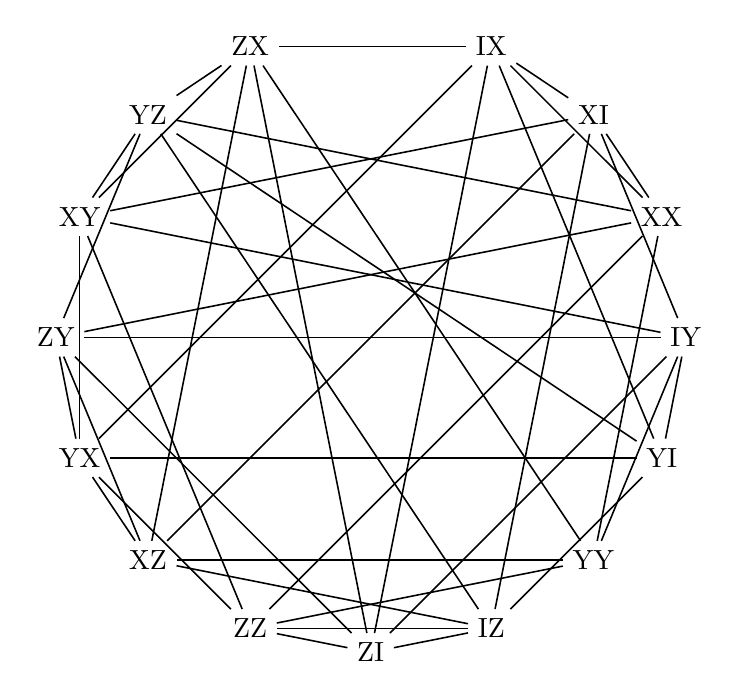
\begin{tikzpicture}
            \node[] (IX) at (2*0.7653668647301797 , 2* 1.847759065022573)    {IX};
            \node[] (XI) at (2*1.4142135623730951 , 2*1.414213562373095)    {XI};
            \node[] (XX) at (2*1.8477590650225735 , 2*0.7653668647301796)   {XX};
            \node[] (IY) at (2*2.0, 0.0)                                  {IY};
            \node[] (YI) at (2* 1.847759065022573 , 2*-0.7653668647301808)   {YI};
            \node[] (YY) at (2* 1.4142135623730947 , 2*-1.4142135623730954)  {YY};
            \node[] (IZ) at (2* 0.76536686473018 , 2*-1.8477590650225733)    {IZ};
            \node[] (ZI) at (2* 0 , 2*-2.0)                                  {ZI};
            \node[] (ZZ) at (2* -0.7653668647301807 , 2*-1.847759065022573)  {ZZ};
            \node[] (XZ) at (2* -1.4142135623730954 , 2*-1.414213562373095)  {XZ};
            \node[] (YX) at (2* -1.8477590650225737 , 2*-0.7653668647301793) {YX};
            \node[] (ZY) at (2* -2.0 , 2*0)                                  {ZY};
            \node[] (XY) at (2* -1.8477590650225735 , 2*0.7653668647301798)  {XY};
            \node[] (YZ) at (2* -1.414213562373095 , 2*1.4142135623730951)   {YZ};
            \node[] (ZX) at (2* -0.7653668647301795 , 2*1.8477590650225735)  {ZX};

            \draw[line width=0.2mm, black ,-] (IX) -- (ZX) ;
            \draw[line width=0.2mm, black ,-] (IX) -- (YX) ;
            \draw[line width=0.2mm, black ,-] (IX) -- (ZI) ;
            \draw[line width=0.2mm, black ,-] (IX) -- (YI) ;
            \draw[line width=0.2mm, black ,-] (IX) -- (XX) ;
            \draw[line width=0.2mm, black ,-] (IX) -- (XI) ;

            \draw[line width=0.2mm, black ,-] (XI) -- (XY) ;
            \draw[line width=0.2mm, black ,-] (XI) -- (XZ) ;
            \draw[line width=0.2mm, black ,-] (XI) -- (IZ) ;
            \draw[line width=0.2mm, black ,-] (XI) -- (IY) ;
            \draw[line width=0.2mm, black ,-] (XI) -- (XX) ;

            \draw[line width=0.2mm, black ,-] (XX) -- (YZ);
            \draw[line width=0.2mm, black ,-] (XX) -- (ZY);
            \draw[line width=0.2mm, black ,-] (XX) -- (ZZ);
            \draw[line width=0.2mm, black ,-] (XX) -- (YY);

            \draw[line width=0.2mm, black ,-] (IY) -- (XY);
            \draw[line width=0.2mm, black ,-] (IY) -- (ZY);
            \draw[line width=0.2mm, black ,-] (IY) -- (ZI);
            \draw[line width=0.2mm, black ,-] (IY) -- (YY);
            \draw[line width=0.2mm, black ,-] (IY) -- (YI);

            \draw[line width=0.2mm, black ,-] (YI) -- (YZ);
            \draw[line width=0.2mm, black ,-] (YI) -- (YX);
            \draw[line width=0.2mm, black ,-] (YI) -- (IZ);

            \draw[line width=0.2mm, black ,-] (YY) -- (ZX);
            \draw[line width=0.2mm, black ,-] (YY) -- (XZ);
            \draw[line width=0.2mm, black ,-] (YY) -- (ZZ);

            \draw[line width=0.2mm, black ,-] (IZ) -- (YZ);
            \draw[line width=0.2mm, black ,-] (IZ) -- (XZ);
            \draw[line width=0.2mm, black ,-] (IZ) -- (ZZ);
            \draw[line width=0.2mm, black ,-] (IZ) -- (ZI);

            \draw[line width=0.2mm, black ,-] (ZI) -- (ZX);
            \draw[line width=0.2mm, black ,-] (ZI) -- (ZY);
            \draw[line width=0.2mm, black ,-] (ZI) -- (ZZ);
            
            \draw[line width=0.2mm, black ,-] (ZZ) -- (XY);
            \draw[line width=0.2mm, black ,-] (ZZ) -- (YX);
        

            \draw[line width=0.2mm, black ,-] (XZ) -- (ZX);
            \draw[line width=0.2mm, black ,-] (XZ) -- (ZY);
            \draw[line width=0.2mm, black ,-] (XZ) -- (YX);

            \draw[line width=0.2mm, black ,-] (YX) -- (XY);
            \draw[line width=0.2mm, black ,-] (YX) -- (ZY);

            \draw[line width=0.2mm, black ,-] (ZY) -- (YZ);

            \draw[line width=0.2mm, black ,-] (XY) -- (ZX);
            \draw[line width=0.2mm, black ,-] (XY) -- (YZ);

            \draw[line width=0.2mm, black ,-] (ZX) -- (YZ);
        \end{tikzpicture}
        \begin{tikzpicture}
    \node[] (IX) at (2*0.7653668647301797 , 2* 1.847759065022573)    {IX};
    \node[] (XI) at (2*1.4142135623730951 , 2*1.414213562373095)    {XI};
    \node[] (XX) at (2*1.8477590650225735 , 2*0.7653668647301796)   {XX};
    \node[] (IY) at (2*2.0, 0.0)                                  {IY};
    \node[] (YI) at (2* 1.847759065022573 , 2*-0.7653668647301808)   {YI};
    \node[] (YY) at (2* 1.4142135623730947 , 2*-1.4142135623730954)  {YY};
    \node[] (IZ) at (2* 0.76536686473018 , 2*-1.8477590650225733)    {IZ};
    \node[] (ZI) at (2* 0 , 2*-2.0)                                  {ZI};
    \node[] (ZZ) at (2* -0.7653668647301807 , 2*-1.847759065022573)  {ZZ};
    \node[] (XZ) at (2* -1.4142135623730954 , 2*-1.414213562373095)  {XZ};
    \node[] (YX) at (2* -1.8477590650225737 , 2*-0.7653668647301793) {YX};
    \node[] (ZY) at (2* -2.0 , 2*0)                                  {ZY};
    \node[] (XY) at (2* -1.8477590650225735 , 2*0.7653668647301798)  {XY};
    \node[] (YZ) at (2* -1.414213562373095 , 2*1.4142135623730951)   {YZ};
    \node[] (ZX) at (2* -0.7653668647301795 , 2*1.8477590650225735)  {ZX};

    \draw[line width=0.2mm, green ,-] (IX) -- (XX) ;
    \draw[line width=0.2mm, green ,-] (IX) -- (XI) ;
    \draw[line width=0.2mm, green ,-] (XI) -- (XX) ;

    \draw[line width=0.2mm, green ,-] (IY) -- (YY);
    \draw[line width=0.2mm, green ,-] (IY) -- (YI);
    \draw[line width=0.2mm, green ,-] (YI) -- (YY);

    \draw[line width=0.2mm, green ,-] (IZ) -- (ZZ);
    \draw[line width=0.2mm, green ,-] (IZ) -- (ZI);
    \draw[line width=0.2mm, green ,-] (ZI) -- (ZZ);

    \draw[line width=0.2mm, green ,-] (XZ) -- (YX);
    \draw[line width=0.2mm, green ,-] (XZ) -- (ZY);
    \draw[line width=0.2mm, green ,-] (YX) -- (ZY);


    \draw[line width=0.2mm, green ,-] (XY) -- (ZX);
    \draw[line width=0.2mm, green ,-] (XY) -- (YZ);
    \draw[line width=0.2mm, green ,-] (ZX) -- (YZ);
\end{tikzpicture}
        }
    \caption{
        Left: Compatible graph of 2-qubit system Pauli-strings. 
        Each edge indicates commuting relationship between the two ends.
        The edges in the figure weighted zero, and edges between disconnected nodes
        are weighted as 1.
        Right:
        The figure was refered from Kurita et al. 2023, redrawed by the author\cite{kurital_2023}.
    }
    \label{fig:compatible_graph_example_2qubits}
\end{figure}
%\begin{figure}[ht]
%    \centering
%        \begin{tikzpicture}
    \node[] (IX) at (2*0.7653668647301797 , 2* 1.847759065022573)    {IX};
    \node[] (XI) at (2*1.4142135623730951 , 2*1.414213562373095)    {XI};
    \node[] (XX) at (2*1.8477590650225735 , 2*0.7653668647301796)   {XX};
    \node[] (IY) at (2*2.0, 0.0)                                  {IY};
    \node[] (YI) at (2* 1.847759065022573 , 2*-0.7653668647301808)   {YI};
    \node[] (YY) at (2* 1.4142135623730947 , 2*-1.4142135623730954)  {YY};
    \node[] (IZ) at (2* 0.76536686473018 , 2*-1.8477590650225733)    {IZ};
    \node[] (ZI) at (2* 0 , 2*-2.0)                                  {ZI};
    \node[] (ZZ) at (2* -0.7653668647301807 , 2*-1.847759065022573)  {ZZ};
    \node[] (XZ) at (2* -1.4142135623730954 , 2*-1.414213562373095)  {XZ};
    \node[] (YX) at (2* -1.8477590650225737 , 2*-0.7653668647301793) {YX};
    \node[] (ZY) at (2* -2.0 , 2*0)                                  {ZY};
    \node[] (XY) at (2* -1.8477590650225735 , 2*0.7653668647301798)  {XY};
    \node[] (YZ) at (2* -1.414213562373095 , 2*1.4142135623730951)   {YZ};
    \node[] (ZX) at (2* -0.7653668647301795 , 2*1.8477590650225735)  {ZX};

    \draw[line width=0.2mm, green ,-] (IX) -- (XX) ;
    \draw[line width=0.2mm, green ,-] (IX) -- (XI) ;
    \draw[line width=0.2mm, green ,-] (XI) -- (XX) ;

    \draw[line width=0.2mm, green ,-] (IY) -- (YY);
    \draw[line width=0.2mm, green ,-] (IY) -- (YI);
    \draw[line width=0.2mm, green ,-] (YI) -- (YY);

    \draw[line width=0.2mm, green ,-] (IZ) -- (ZZ);
    \draw[line width=0.2mm, green ,-] (IZ) -- (ZI);
    \draw[line width=0.2mm, green ,-] (ZI) -- (ZZ);

    \draw[line width=0.2mm, green ,-] (XZ) -- (YX);
    \draw[line width=0.2mm, green ,-] (XZ) -- (ZY);
    \draw[line width=0.2mm, green ,-] (YX) -- (ZY);


    \draw[line width=0.2mm, green ,-] (XY) -- (ZX);
    \draw[line width=0.2mm, green ,-] (XY) -- (YZ);
    \draw[line width=0.2mm, green ,-] (ZX) -- (YZ);
\end{tikzpicture}
%        \caption{
%            Example of mutually commuting partition of Fig (\ref{fig:compatible_graph_example_2qubits})
%            }
%        \label{fig:compatible_graph_example_2qubits-commuting-set}
%\end{figure}

Kurita et al used a graph partitioning Hamiltonian and 
constructed sequetial clique extracting algorithm.
The compatible graph modeled as binary, 0 and 1, weighted 
complete graph by edges of commutation are marked as 0 
and the anti-commutation ones are marked as 1.
Basic procedure of Kurita et al is 

\begin{enumerate}
    \item Extract max-clique set, $P_i$, from the compatible graph.
    \item Delete the nodes which were extracted from the step 1 from the graph.
    \item Repeat until there is no remaining node after step 2.
\end{enumerate}.

The mutually commuting partitions are constructed 
by each max-cliques, $\{P_i\}_{i=1}^N$. 
The mutually commutation relationship is guaranteed by the next 
Hamiltonian, quadratic ising model.

\begin{equation}
    \mathcal{H} = -\sum_i x_i + \sum_{i >j} x_i xj
\end{equation}

The first term, $-\sum_i x_i$, reduces the state energy 
proportional to a number of nodes in the clique.
The second term, $\sum_{i >j} x_i xj$ raises the state energy
as much of the number of the anti-commuting terms in the sample.
At each step, the clique searching was conducted by stimulated annealing chip provided by Fujititu. 


%\section{Pauli Frame}
%
%In the evolution circuit of the specific Pauli string, the circuit consist of several manipulation terms by the configuration of the CNOT gates.
%
%Even if, there are $N'$ number of mutually commuting Pauli-strings, 
%the single operation step evolution only possible for $N$ number of the strings. 
%$N$ is a number of qubits in the algorithm.


\section{Axis transformation weight}

The main idea of Kurita et al allow us to find 
mutually commuting partition of the given 
Hamiltonian set. 
However, there are some degeneracy in extracting cliques 
from the pauli-graph of the given Hamiltonian.

Consider the next Pauli graph.

\begin{center}
    \begin{tikzpicture}
        \node[regular polygon, regular polygon sides=5, minimum size=3cm] at (0,0) (A) {};
        \node[circle, fill=white, draw=black] (zx) at (A.corner 1) {ZX};
        \node[circle, fill=white, draw=black] (xz) at (A.corner 2) {XZ};
        \node[circle, fill=white, draw=black] (iy) at (A.corner 3) {IY};
        \node[circle, fill=white, draw=black] (yi) at (A.corner 4) {YI};
        \node[circle, fill=white, draw=black] (yy) at (A.corner 5) {YY};

        \draw[line width=0.4mm, black ,-] (xz) -- (zx) ;
        \draw[line width=0.4mm, black ,-] (xz) -- (yy) ;
        \draw[line width=0.4mm, black ,-] (zx) -- (yy) ;
        \draw[line width=0.4mm, black ,-] (yy) -- (iy) ;
        \draw[line width=0.4mm, black ,-] (yy) -- (yi) ;
        \draw[line width=0.4mm, black ,-] (iy) -- (yi) ;
        %\foreach \i[evaluate={\j=int(17-\i)}] in {2,...,15}
        %    \node[circle, fill=white, draw=black, ultra thick] (\j) at (A.corner \i) {$B_{\j}$};
        % Line
        %\foreach \i[evaluate={\j=int(int(\i+1) - int((\i+1)/16))}] in {0, ..., 15}
        %    \draw[line width=0.1mm, black ,-] (\i) -- (\j);
    \end{tikzpicture}
\end{center}

We have two possible partitions in the optimization process.

\begin{center}
    \begin{tikzpicture}
        \node[regular polygon, regular polygon sides=5, minimum size=3cm] at (0,0) (A) {};
        \node[circle, fill=white, draw=black] (zx) at (A.corner 1) {ZX};
        \node[circle, fill=white, draw=black] (xz) at (A.corner 2) {XZ};
        \node[circle, fill=white, draw=black] (iy) at (A.corner 3) {IY};
        \node[circle, fill=white, draw=black] (yi) at (A.corner 4) {YI};
        \node[circle, fill=white, draw=black] (yy) at (A.corner 5) {YY};

        \draw[line width=0.4mm, black ,-] (xz) -- (zx) ;
        \draw[line width=0.4mm, black ,-] (yy) -- (iy) ;
        \draw[line width=0.4mm, black ,-] (yy) -- (yi) ;
        \draw[line width=0.4mm, black ,-] (iy) -- (yi) ;
    \end{tikzpicture}
    \hspace{1cm}
    \begin{tikzpicture}
        \node[regular polygon, regular polygon sides=5, minimum size=3cm] at (0,0) (A) {};
        \node[circle, fill=white, draw=black] (zx) at (A.corner 1) {ZX};
        \node[circle, fill=white, draw=black] (xz) at (A.corner 2) {XZ};
        \node[circle, fill=white, draw=black] (iy) at (A.corner 3) {IY};
        \node[circle, fill=white, draw=black] (yi) at (A.corner 4) {YI};
        \node[circle, fill=white, draw=black] (yy) at (A.corner 5) {YY};

        \draw[line width=0.4mm, black ,-] (xz) -- (zx) ;
        \draw[line width=0.4mm, black ,-] (xz) -- (yy) ;
        \draw[line width=0.4mm, black ,-] (zx) -- (yy) ;
        \draw[line width=0.4mm, black ,-] (iy) -- (yi) ;
    \end{tikzpicture}
\end{center}

These two partition are indistinguishable in binary weighted 
graph suggested by Kurita et al. 
That means, the system has a degeneracy in the ground state.
In general, each intermediate steps we would face such degeneracy 
in the max-clique finding problem.
However, if we consider an additional implementation cost 
on the circuit, we can remove such degeneracy from the process.
The author, Kim, suggested basis transformation weight to the 
Kurita's Hamiltonian.

In 2 qubit system, general evolution operator of length two Pauli-string on circuit would
have next form.

\begin{center}
\begin{quantikz}
    & \gate{B_1} & \ctrl{1}& & \ctrl{1} & \gate{B_1^\dagger}\\
    & \gate{B_2} & \targ{} & \gate{RZ(2\Delta t)}& \targ{} & \gate{B_2^\dagger}\\
\end{quantikz}
\end{center}

By the axis of the rotation, 
the basis transformation gates rotate the qubit axes.
However, some cases intermediate gates between 
rotation gates are not necessary to exist.
If the nested rotation axes, mutually commuting 
by the method of implementation we can ignore the basis transformation circuit.
See an example and details in \textit{Pauli-Frame}.

Two parameters could be considered in the problem.

\begin{itemize}
    \item Circuit depth
    \item Number of gates 
\end{itemize}

\subsection{Rough implementation of single qubit transformation}

Transformation method to the graph clique problem and
corresponding problem is well established in Kurita et al.

\begin{center}
    \begin{quantikz}
        & \gate{B} &
    \end{quantikz}
     = \begin{quantikz}
         \gate{H} 
    \end{quantikz} or \begin{quantikz}
         \gate{S^\dagger} & \gate{H}
    \end{quantikz}
\end{center}

\begin{definition}{\textbf{Single qubit transformation depth}}
    
    The transformation depth of the nested axes, $A_1, A_2$ is defined as,
    \begin{equation}
        w(\cdot) : P^1 \times P^1 \rightarrow \mathbb{Z}_+
    \end{equation}

    where, $P^1 = \{I, X, Y, Z\}$.
\end{definition}

\begin{center}
    \begin{tabular}{c c c}
        \hline
        Nested Axes & Transformation gate & Transformation Depth\\
        \hline
        A A & $I    $ & 0 \\
        Z X & $H    $ & 1 \\
        Z Y & $S^\dagger H  $  & 2 \\
        X Y & $H S^\dagger H$ & 3\\
    \end{tabular}
\end{center}

Expand them to the multi-qubit Hamiltonian, then 

\begin{equation}
    W(S_i, S_j) := \frac{1}{N} \sum_{k=1}^N w((S_i)_k, (S_j)_k) 
\end{equation}


\begin{equation}
    \mathcal{H} = - \mu_o \sum  Z_i + \mu_1 \sum_{i <j} h_{ij} Z_iZ_j + \mu_2 \sum_{i<j} w_{ij} Z_i Z_j
\end{equation}

where, $h_{ij} \in \{0, 1\}$ and $w_{ij} \in [0, 1]$.

To avoid the reversed energy of the commuting and non-commuting 
states, the prior coefficients, $\mu_0, \mu_1, \mu_2$ must satisfies the next constraints,

\begin{equation}
    \begin{cases}
        || \mu_1 || > N || \mu_0|| \\
        || \mu_0 ||  > \frac{1}{2} N (N-1) || \mu_2||
    \end{cases}
\end{equation}

The transofrmation weight could be differ by the 
basis gate set of th system and implementation unit.
For example, the above construction was based on 
introductory level implementation of time-evolution gate
using RZ, CNOT and Hadamard and S gates. 
However, there are many way to construct the gate.
You can use RX or RY instead of RZ,
simulatneously use two rotation gates,
CZ, CY, or instead of CNOT, or
instead of RZ gate, you can choose phase gate.

\subsection{Pauli-Frame metric}



%------------------------------------------------------
Yet's we even have no idea of quantum advantaged algorithm for TSP problem.
Therefore, in this approach we seperated the problem in to several well-known
, at least come conveience approximation method exists,
problems.

Main idea is same with the Kurita et al's approach however, we combined them with Pauli-Frame 
transformation cost in the partitioning steps.


In the design of the graph optimization Hamiltonian, what is a proper ground state must be considered.
For example, the actual path of each Pauli-strings would be formated after the partition generated.
Then, must the highest weighted edge be cut in partition steps or formation steps?
Answer, even we can find bypass route to avoid such path, it is more appropriate to cut the huge weighted edge
in partition formation step. %이부분 애매모호한데 각잡고 해결해 봅시다.


The main idea is energy split the graph partitioning Hamiltonian by adding basis transformation cost.
See an example case of degenerated situation in Kurita et al.
The next compatible graph has two solution for max-clique extraction.

However, these two configurations are not same 
for the total error reduction in final result including implementation error.

Now, we are considering circuit-depth of the evolution circuit.
What is a more suitable for depth reduction in this case?

Basis transform cancelling and multi-rotating pauli-frame could be a good
estimation measure.

Considering a two 

by the basis of each qubit, the transform layer depth is 0-3.
in 0- 1 cases precisely defined CNOT gate allow more reduction of circuit.

See, Pauli-frame optimization.

Now, our job is applying such configuration in clique optimization.


\textbf{insist} With mutually commuting partition, the degree of the freedom in 
Pauli-frame in optimization process is greatly reduced.


The heuristhic assumption was if the most high cost edge exists in node set. 
It requires other edges than the lower cost edges to find minimum cost path travling all nodes.



\textbf{Note: Idea}
The problem of Pauli-frame optimization is that it is a Traveling Shopper problem which is more complex and higher 
NP-Problem of TSP(Traveling Saleman Problem).
The Pauli-frame optimization automatically satisfies the muttually commuting order optimization, since 
a Pauli-frame in steps represents the mutually commuting Pauli-strings groups. 
More precisely, Pauli-frame represent the simulatneously possible pauli-strings 
to be implemented on single operation step. 
Optimizing the Pauli-frame is already considering Basis-transform cost.


What if the pre-condition that the given pauli-strings are mutually commuting sets?

\section{Krylov transformation}

Krylov method is a method of change the basis order by the significant of system evolution and drop the low-affection terms to reduce the size of the quantum system.

\subsection{Other techniques}

\section{VQE method and evolution}